%
% One column figure
%-----------------------------------------------------------
   \begin{figure}
   \centering
\tikzstyle{smallfig}=[scale=0.25]
   %
\begin{tikzpicture}[style=smallfig]
\draw [fill=lightgray!20, pattern=north west lines, 
   pattern color=red] (0, 4) rectangle (4, 6);
\draw [fill=lightgray!20, pattern=north west lines, 
   pattern color=red] (4, 0) rectangle (6, 4);
\draw [fill=lightgray!20, pattern=north west lines, 
   pattern color=red] (0, -2) rectangle (4, 0);

\draw[thin,->] (-2,0) -- (6,0) node[right] {$\hat{x}$};
\draw[thin,->] (0,-2) -- (0,6) node[above] {$\hat{y}$};

\draw[dashed,thin,-] (-2,4) -- (6,4);
\draw[dashed,thin,-] (4,-2) -- (4,6);
\fill (0,4) circle (5pt) node[below left] {$1$};
\fill (4,0) circle (5pt) node[below right] {$1$};
\end{tikzpicture}
\quad
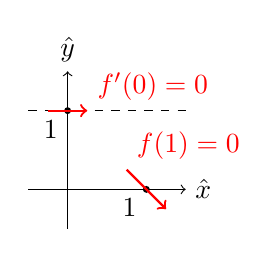
\begin{tikzpicture}[style=smallfig]
\draw[thin,->] (-2,0) -- (6,0) node[right] {$\hat{x}$};
\draw[thin,->] (0,-2) -- (0,6) node[above] {$\hat{y}$};

\draw[dashed,thin,-] (-2,4) -- (6,4);
\fill (0,4) circle (5pt) node[below left] {$1$};
\fill (4,0) circle (5pt) node[below left] {$1$};

\draw[thick,->, red] (-1,4) -- (1,4) node[above right] {$f^\prime(0)=0$};
\draw[thick,->, red] (3,1) node[above right] {$f(1)=0$} -- (5,-1);
\end{tikzpicture}
\quad
\begin{tikzpicture}[style=smallfig]
\draw[thin,->] (-2,0) -- (6,0) node[right] {$\hat{x}$};
\draw[thin,->] (0,-2) -- (0,6) node[above] {$\hat{y}$};

\fill (0,4) circle (5pt) node[below left] {$1$};
\fill (4,0) circle (5pt) node[below left] {$1$};

\begin{scope}[thick, decoration={
    markings,
    mark=at position 0.5 with {\arrow{>}}}
    ] 

    \draw[postaction={decorate}] (0,4) to[out=0,in=100] (4,0);
    \draw[postaction={decorate}] (0,4) -- (4,0);
\end{scope}
\end{tikzpicture}
   %
   \caption{Showing the how the constraints on $f$ define its shape
   in $[0,1] \times [0,1]$. The first picture shows the regione where $f$
   can lay, the middle one shows tangent in $x=0$ and the condition
   of crossing in $(1,0)$. The rightmost picture shows possible
   shapes of $f$: note how the concavity cannot be pointing upwards.}
   \label{fig:fshape}
   \end{figure}
%-----------------------------------------------------------
%